\chapter{Background Material}
\label{chap:background}
This chapter provides a review of mathematical and theoretical material pertinent to this research.
First, the geometric discretization used in this work is discussed.
Second, the two-phase flow equations are detailed.
Third, the numerical approximations with respect to space, time, and nonlinearities are covered.
Next, the various solution methods currently used to solve the system of discrete governing equations are presented.
And last, an outline of the various means by which domain coupling of thermal-hydraulic safety analysis software has traditionally been achieved is provided.

%-------------------------------------------------------------------------------
%-------------------------------------------------------------------------------
%-------------------------------------------------------------------------------
\section{Geometric Discretization}
\label{sect:geometry}
The first step in any simulation of the thermal-hydraulic behavior of the core of a nuclear reactor is to create a discrete computational representation of the domain.
For this work the computational grid used to represent the physical model is a staggered mesh.
With a staggered mesh the domain is divided into two overlapping meshes.
There is one mesh comprised of continuity volumes and another comprised of momentum flow paths, as shown in \fig{fig:staggered_mesh}.
Thermodynamic variables are defined as constant over the continuity volumes, while momenta are defined as constant over momentum flow paths.
The boundaries of the continuity volumes align with the center of the momentum flow paths.

\begin{figure}[ht!]
\centering
\tikzsetnextfilename{images/staggered_mesh_eps}
\begin{tikzpicture}
\draw (-3,0) rectangle +(1,5);
\draw (0,0) rectangle +(1,1) (0,1) rectangle +(1,1) (0, 2) rectangle +(1,1) (0,3) rectangle +(1,1) (0,4) rectangle +(1,1);
\draw[dashed] (3,-0.5) rectangle +(1,1) (3,0.5) rectangle +(1,1) (3,1.5) rectangle +(1,1) (3, 2.5) rectangle +(1,1) (3,3.5) rectangle +(1,1) (3,3.5) rectangle +(1,1) (3, 4.5) rectangle +(1,1) ;
\draw[dashed] (-3,0) -- (4,0);
\draw[dashed] (-3,5) -- (4,5);
\draw (-2.5,-1) node {Channel};
\draw (0.5,-1) node {Continuity};
\draw (0.5,-1.5) node {Volume};
\draw (3.5,-1) node {Momentum};
\draw (3.5,-1.5) node {Flow Path};
\end{tikzpicture}
\caption{A representation of the staggered mesh.}
\label{fig:staggered_mesh}
\end{figure}

The geometric modeling framework in this work involves two primary components: sections and subchannels.
The total axial height of the problem is divided into sections.
Each section is defined by two bounding elevations and a spatial discretization of that span into discrete non-overlapping axial segments that represent the axial spacing of the continuity volumes.
The total number of continuity volumes in a given subchannel is one less than the number of momentum flow paths in that subchannel.
The particular axial discretization of a given section is independent from that of the other sections.

Within a given section, subchannels are defined.
A subchannel inherits the axial discretization of its parent section.
The number of subchannels in a given section is independent of the number of subchannels in other the sections.
Each continuity volume and momentum flow path has an associated cross-sectional area, $A_{c}$ and $A_{m}$, respectively. 
These cross-sectional areas can vary from volume to volume and from flow path to flow path.
By definition the momentum flow paths do not contain mass or energy.

It is also possible to model multi-dimensional flow through the definition of transverse flow paths that connect two subchannels within a given section.
The transverse flow paths are orthogonal to the axial flow direction.
Additionally, it is permissible to have the axial flow from a single subchannel split into multiple subchannels in an adjacent section.
This flow splitting is only permitted at section boundaries.
By using these features geometrically complex models can be created.
An example of a model that includes these different geometric characteristics is given in \fig{fig:complex_geometry}.

\begin{figure}[ht!]
\centering
\tikzsetnextfilename{images/complex_geometry_pdf}
\begin{tikzpicture}
%\draw [thick] (-2,-2) rectangle (-1,2);
%\draw [thick] (1,-2) rectangle (2,2);
%\draw [thick] (-0.5,3) rectangle (0.5,7);
%\draw [thick] (-0.5,-7) rectangle (0.5,-3);

%Section 1
\draw [thick] (-0.25,-6) rectangle (0.25,-5.25);
\draw [thick] (-0.4,-5.25) rectangle (0.4,-4.5);
\draw [thick] (-0.5,-4.5) rectangle (0.5,-3.75);
\draw [thick] (-0.3,-3.75) rectangle (0.3,-3);

%Section 2: left then right
\draw [thick] (-1.75,-2) rectangle (-1.25,-1);
\draw [thick] (-1.6,-1) rectangle (-1.4,0);
\draw [thick] (-2,-0) rectangle (-1,1);
\draw [thick] (-1.75,1) rectangle (-1.25,2);

\draw [thick] (1.1,-2) rectangle (1.9,-1);
\draw [thick] (1.1,-1) rectangle (1.9,0);
\draw [thick] (1.25,0) rectangle (1.75,1);
\draw [thick] (1.3,1) rectangle (1.7,2);

%Section 3
\draw [thick] (-0.25,3) rectangle (0.25,3.8);
\draw [thick] (-0.5,3.8) rectangle (0.5,4.6);
\draw [thick] (-0.4,4.6) rectangle (0.4,5.4);
\draw [thick] (-0.5,5.4) rectangle (0.5,6.2);
\draw [thick] (-0.25,6.2) rectangle (0.25,7);
\draw [thick] (-0.25,7) rectangle (0.25,7.8);

%Flow lines
\draw [dashed] (-1.5,2.5) -- (1.5,2.5);
\draw [dashed](-1.5,-2.5) -- (1.5,-2.5);
\draw [dashed,<-] (0,3) -- (0,2.5);
\draw [dashed,->] (-1.5,2.5) -- (-1.5,2);
\draw [dashed,->] (1.5,2.5) -- (1.5,2);
\draw [dashed,->] (0,-2.5) -- (0,-3);
\draw [dashed,<-] (-1.5,-2) -- (-1.5,-2.5);
\draw [dashed,<-] (1.5,-2) -- (1.5,-2.5);

\draw [dashed, <->] (-1.25,-1.5) -- (1.1,-1.5);
\draw [dashed, <->] (-1.4,-0.5) -- (1.1,-0.5);
\draw [dashed, <->] (-1,0.5) -- (1.25,0.5);
\draw [dashed, <->] (-1.25,1.5) -- (1.3,1.5);	
\foreach \y/\ytext in {-4.5/ 1,0/ 2,5.5/ 3}
	\draw (2,\y) node [anchor=west] {Section $\ytext$};
\end{tikzpicture}
\caption{A model with transverse flow.}
\label{fig:complex_geometry}
\end{figure}

%-------------------------------------------------------------------------------
%-------------------------------------------------------------------------------
%-------------------------------------------------------------------------------
\section{Two-Phase Flow Equations}
\label{sect:two_phase_flow}
The primary purpose of subchannel analysis codes is to determine fuel integrity via evaluation of effective core cooling during postulated NPP accidents, such as a LOCA.
This requires accurate modeling the heat transfer between the coolant and the fuel. 
During postulated accidents, the coolant, H$_2$O, can undergo phase-change.
There are several formulations of the governing conservation equations of fluid mechanics used to predict the thermal-hydraulic response of the nuclear reactor core to transient plant conditions.
To model the complex phenomenon of phase-change, the governing equations for the fluid mechanics within the core will be those of a multicomponent fluid \cite{Drew1998}.
In particular, they are a subcategory of two-phase flow \cite{Todreas2011, Stewart1984, Ishii1984}.
This section will discuss both the assumptions used and the final governing equations obtained for modeling two-phase flow.

%-------------------------------------------------------------------------------
%-------------------------------------------------------------------------------
%-------------------------------------------------------------------------------
\subsection{Assumptions}
\label{subsect:assumptions}

The governing equations of fluid-mechanics provide extensive information about fluid behavior.
However, one of the basic assumptions of subchannel analysis is that the exact spatial behavior of the coolant is not of direct interest; as such, the average behavior of the fluid is what is modeled.
Given the multi-phase nature of the coolant, there are various ways in which the interactions between the various phases can be modeled.
For the conditions encountered in a commercial nuclear reactor core, certain assumptions can be made to reduce the complexity of the physics involved.
This section will discuss: the technique used to obtain equations for averaged quantities, the manner in which the multi-phase nature of the coolant is dealt with, and the general assumptions used reduce the complexity of the physics.

The first simplification is that the exact topology of the interface between the coolant phases need not be known to model the fluid mechanics.
Since the exact deterministic behavior of the phasic-interface is no longer necessary, the governing equations can be subjected to averaging procedures to produce conservation laws for averaged quantities.
There are several averaging techniques that have been used to produce the conservation laws for two-phase flow: spatial, temporal, and ensemble averaging \cite{Drew1998, Todreas2011}.
Each of these techniques has its own physical interpretation and mathematical formulation.
The formulation used in this work is area averaging, a particular form of spatial averaging.
In the area-averaged formulation the governing equations are averaged over the cross-sectional area.

The second simplification regards the manner in which the multi-phase nature of the coolant is treated.
The particular formulation of the two-phase flow equations used in this work is commonly referred to as a ``two-phase, three-field formulation."
While this designation comes from the three water fields that are modeled by the software, the software also models \ncg{} fields that are mixed with the steam.
To simulate the behavior of in-core fluid dynamics during accident scenarios more accurately, the liquid and the gaseous phases are each divided into two distinct fields.
The two fields of the liquid phase are a continuous liquid field and an entrained liquid droplet field.
The gaseous phase is composed of a mixture of a \ncg{} field and a water-vapor field. 
This ability to track the different fields within a phase provides two important benefits to safety analysis: the ability to account for the effects of \ncgs{} on condensation and the ability to model the effects of the entrained liquid droplets on heat transfer.
The benefits of modeling the entrained liquid field have inspired the developers of the French CATHARE software to migrate to a similar three-field formulation in the next version of their software \cite{Emonot2011}.

Given the four fields of interest, there are twelve conservation equations in axial flow, one each for the mass, momentum, and energy of each of the four fields.
Additional closure relationships are necessary to describe the interactions between the various fields and their interfacial transfer terms.
These equations allow for a description of the time-dependent behavior of the in-core fluid.
However, assumptions are made to reduce the number of required conservation laws and the number of corresponding closure relationships.
The following is a list of the assumptions that are made to reduce the complexity of the governing equations.

\begin{itemize}
\item{
Thermodynamic and pressure equilibrium exists between the continuous liquid field and the entrained liquid field.
The basis for this assumption is that, while the entrained droplets are being modeled by a separate set of governing equations than those of the continuous liquid field, the droplets are constantly entraining from and depositing to the continuous liquid field. 
}
\item{
The liquid and gaseous phases are assumed to be in pressure equilibrium with the interface between the phases.
The basis for this assumption is that the inter-phase dynamics at the interface are negligible when compared to the bulk flow dynamics.
}
\item{The \ncg{} and steam components of the gaseous phase are in mechanical equilibrium.}
\item{The two components of the gaseous phase obey Dalton's Law.}
\item{The two components of the gaseous phase are in thermal equilibrium.}
\item{
The viscous dissipation of momentum in the axial flow direction and the associated generation of energy are neglected.
This assumption is made because the simulations of interest are dominated by inertial, not viscous, forces so that the neglected terms would be small compared to other terms in the calculations.
}
\item{
The wall-shear effects of viscosity are accounted for via empirically based friction correlations.
}
\item{
The primary positive flow direction is counter to the gravity vector, which will be referred to as the axial flow direction. This vertically oriented coordinate system was chosen to accommodate the vertical core design of NPPs.}
\item{
The mechanical energy of the phases is neglected in the conservation of energy. 
The assumption is that in the simulations of interest the mechanical energy term is negligible.
}
\item{
The effects of turbulence are only incorporated through the closure relationships used for wall friction and wall heat transfer.
}
\end{itemize}

%-------------------------------------------------------------------------------
%-------------------------------------------------------------------------------
%-------------------------------------------------------------------------------
\subsection{Governing Equations}
\label{subsect:governing_equations}

Following the application of the above assumptions, nine governing partial differential equations (PDEs) for axial flow remain: four for mass conservation, two for energy conservation, and three for momentum conservation.
The details of this system of PDEs are discussed below.

%-------------------------------------------------------------------------------
%-------------------------------------------------------------------------------
%-------------------------------------------------------------------------------
\subsubsection{Conservation of Mass Equations}
\label{subsubsect:mass_equations}

There are four equations that represent the conservation of mass, one each for the vapor \eqref{eqn:conservation_of_vap}, \ncg{} \eqref{eqn:conservation_of_ncg}, continuous liquid  \eqref{eqn:conservation_of_liq}, and entrained liquid \eqref{eqn:conservation_of_ent} fields.

\begin{IEEEeqnarray}{rCl}
\label{eqn:conservation_of_ncg}
\frac{\partial \left(\alpha_g \rho_{n}\right) }{\partial t } + \nabla \cdot \left( \alpha_g \rho_{n} \vec{u}_g \right) & = & \dot{s}^{'''}_{m,n} \\
\label{eqn:conservation_of_vap}
\frac{\partial \left(\alpha_g \rho_v \right)}{\partial t } + \nabla \cdot \left( \alpha_g \rho_v \vec{u}_g \right)         & = & \dot{\Gamma}^{'''} + \dot{s}^{'''}_{m,v} \\
\label{eqn:conservation_of_liq}
\frac{\partial \left(\alpha_l \rho_l \right)}{\partial t } + \nabla \cdot \left( \alpha_l \rho_l \vec{u}_l \right)         & = & -(1-\eta)\dot{\Gamma}^{'''} - \dot{\Upsilon}^{'''} + \dot{s}^{'''}_{m,l} \\
\label{eqn:conservation_of_ent}
\frac{\partial \left(\alpha_e \rho_l \right)}{\partial t } + \nabla \cdot \left( \alpha_e \rho_l \vec{u}_e \right)         & = & -\eta\dot{\Gamma}^{'''} + \dot{\Upsilon}^{'''}+ \dot{s}^{'''}_{m,e}
\end{IEEEeqnarray}

The left-hand sides of \eqref{eqn:conservation_of_ncg} -- \eqref{eqn:conservation_of_ent} represent the Lagrangian derivative for the given field.
The terms on the right-hand side represent the volumetric rate of the inter-field ($\dot{\Upsilon}^{'''}$), inter-phase ($\dot{\Gamma}^{'''}$), and external ($\dot{s}^{'''}_{m,\phi}$) mass transfer.
Since there are two liquid fields, the rate of mass transfer between the water-vapor field and the liquid fields, $\dot{\Gamma}^{'''}$, is apportioned between the continuous liquid field and the entrained liquid field.
The relationship between the phasic mass transfer terms is given by \eqref{eqn:apportionment_of_mass_transfer}, where $\eta$ is an apportionment factor. 

\begin{equation}
\label{eqn:apportionment_of_mass_transfer}
\dot{\Gamma}^{'''} = \eta \dot{\Gamma}^{'''} + (1 - \eta)\dot{\Gamma}^{'''}
\end{equation}

The inter-field transfer of mass occurs only between the continuous and entrained liquid fields, \eqref{eqn:entrainment_deentrainment}.

\begin{equation}
\label{eqn:entrainment_deentrainment}
\dot{\Upsilon}^{'''}_l + \dot{\Upsilon}^{'''}_e = 0
\end{equation}

Within the conservation of mass equations several assumptions from \sect{subsect:assumptions} are evident.
The mechanical equilibrium of the \ncg{} and the vapor field manifests itself in the singular velocity for the two gaseous fields: $\vec{u}_g$, where the $g$ subscript denotes the total gaseous phase.
Dalton's Law allows the two components of the gaseous phase to occupy the same volume, thus providing for a singular volume fraction, $\alpha_g$.
The thermodynamic equilibrium of the two liquid fields results in only one liquid density, $\rho_l$.

%-------------------------------------------------------------------------------
%-------------------------------------------------------------------------------
%-------------------------------------------------------------------------------
\subsubsection{Conservation of Energy Equations}
\label{subsubsect:energy_equations}

In addition to the conservation of mass equations there are conservation of energy equations for each of the two phases, \eqref{eqn:con_energy_gas} -- \eqref{eqn:con_energy_liq}.

\begin{IEEEeqnarray}{rCl}
\label{eqn:con_energy_gas}
\frac{\partial \left( \alpha_g \rho_g h_g \right)}{\partial t } + \nabla \cdot \left(  \alpha_g \rho_g h_g \vec{u}_g \right) & =& \nonumber \\
\dot{\Gamma}^{'''} h^{'}_v + \dot{q}^{'''}_{i,v} + \dot{q}^{'''}_{n,l}  + \dot{q}^{'''}_{w,g} + \alpha_g\frac{\partial P}{\partial t} + \dot{s}^{'''}_{h,g}  & &\\
\label{eqn:con_energy_liq}
\frac{\partial \left( (1 - \alpha_g) \rho_l h_l \right) }{\partial t } + \nabla \cdot \left( \alpha_l \rho_l h_l \vec{u}_l \right) + \nabla \cdot \left( \alpha_e \rho_l h_l \vec{u}_e \right)& = & \nonumber \\
-\dot{\Gamma}^{'''} h^{'}_l + \dot{q}^{'''}_{i,l} - \dot{q}^{'''}_{n,l}  + \dot{q}^{'''}_{w,l} + (1 - \alpha_g) \frac{\partial P}{\partial t} + \dot{s}^{'''}_{h,l}  & &
\end{IEEEeqnarray}

The conservation of energy equations used in this work are formulated such that the conserved quantities are the phasic enthalpies, $\alpha_{\phi} \rho_{\phi} h_{\phi}$, where $\phi$ represents either either the gaseous or the liquid phase.
Under the assumption of thermodynamic equilibrium for the two liquid fields, there is a single enthalpy for the two liquid fields.
The gaseous phasic enthalpy, however, is defined according to \eqref{eqn:gaseous_enthalpy}.

\begin{equation}
\label{eqn:gaseous_enthalpy}
\rho_g h_g = \rho_v h_v + \rho_n h_n
\end{equation}

The various terms on the right hand sides of \eqref{eqn:con_energy_gas} and \eqref{eqn:con_energy_liq} are defined as follows:

\begin{itemize}
\item{
$\dot{\Gamma}^{'''} h^{'}_{\phi}$:
 energy transfer rate due to the phase change of water.
 The effective enthalpies, $h^{'}_{\phi}$, are dependent upon the mechanism of phase change.
}
\item{
$\dot{q}^{'''}_{i,\phi}$:
energy transfer rate between the liquid and vapor fields and the saturated interface.
}
\item{
$\dot{q}^{'''}_{n,l}$:
energy transfer rate between the liquid fields and the \ncgs{}.
}
\item{
$\dot{q}^{'''}_{w,\phi}$:
 energy transfer rate between the solid-structures and a given phase.
}
\item{
$\alpha_{\phi} \frac{\partial P}{\partial t}$:
 pressure work done by a given phase $\phi$.
 The liquid volume fraction is the sum of the volume fractions of the continuous and the entrained liquid fields.
}
\item{
$\dot{s}^{'''}_{h,\phi}$:
 energy transfer rate between an external source and a given phase.
}
\end{itemize}

%-------------------------------------------------------------------------------
%-------------------------------------------------------------------------------
%-------------------------------------------------------------------------------
\subsubsection{Conservation of Momentum Equations}
\label{subsubsect:momentum_equations}

Finally, there are three governing equations for the conservation of momentum: the continuous liquid field \eqref{eqn:con_mom_liq}, the gaseous phase \eqref{eqn:con_mom_gas}, and the entrained liquid droplet field \eqref{eqn:con_mom_ent}.
These equations are expressed in vector notation; however, only axial flow will be detailed below.
The assumed mechanical equilibrium between the two gaseous fields enable the use of a single momentum conservation equation for the net gaseous phase.

\begin{IEEEeqnarray}{rCl}
\label{eqn:con_mom_liq}
\frac{\partial \left( \alpha_l \rho_l \vec{u}_l \right )}{\partial t } + \nabla \cdot \left( \alpha_l \rho_l \vec{u}_l \vec{u}_l \right) & = & \nonumber \\
 -\alpha_l \nabla P + \alpha_l \rho_l \vec{g} - \vec{\tau}^{'}_{w,l} + \vec{\tau}^{'}_{i,gl} - (1 - \eta)\dot{\Gamma}^{'''}\vec{u}^{'} - \dot{\Upsilon}^{'''}\vec{u}^{'} + \dot{s}^{'''}_{p,l} & & \\
\label{eqn:con_mom_gas}
\frac{\partial \left( \alpha_g \rho_g \vec{u}_g \right) }{\partial t } + \nabla \cdot \left( \alpha_g \rho_g \vec{u}_g \vec{u}_g \right) & = & \nonumber \\
 -\alpha_g \nabla P + \alpha_g \rho_g \vec{g} - \vec{\tau}^{'}_{w,g} - \vec{\tau}^{'}_{i,gl} - \vec{\tau}^{'}_{i,ge} + \dot{\Gamma}^{'''}\vec{u}^{'} + \dot{s}^{'''}_{p,g} & & \\
\label{eqn:con_mom_ent}
\frac{\partial \left( \alpha_e \rho_l \vec{u}_e \right) }{\partial t } + \nabla \cdot \left( \alpha_e \rho_l \vec{u}_e \vec{u}_e \right) & = & \nonumber \\
 -\alpha_e \nabla P + \alpha_e \rho_l \vec{g} - \vec{\tau}^{'}_{w,e} + \vec{\tau}^{'}_{i,ge} - \eta \dot{\Gamma}^{'''}\vec{u}^{'} + \dot{\Upsilon}^{'''}\vec{u}^{'} + \dot{s}^{'''}_{p,l} & &
\end{IEEEeqnarray}

The $\rho_g$ used in \eqref{eqn:con_mom_gas} is defined by \eqref{eqn:gaseous_density}.

\begin{equation}
\label{eqn:gaseous_density}
\rho_g = \rho_n + \rho_v
\end{equation}

The material derivative of the fluid momentum is represented by the left-hand sides of \eqref{eqn:con_mom_liq} -- \eqref{eqn:con_mom_ent}.
The right-hand sides represent various surface, boundary, and body forces that act upon the fluid.
The various terms in \eqref{eqn:con_mom_liq} -- \eqref{eqn:con_mom_ent} are described below.

\begin{itemize}
\item{
$\alpha_{\phi} \nabla P$:
pressure gradient acting on field $\phi$.
}
\item{
$\alpha_{\phi} \rho_{\phi} \vec{g}$:
gravity body force acting upon field $\phi$.
}
\item{
$\vec{\tau}^{'}_{w,\phi}$:
 shear forces from contact between field $\phi$ and the subchannel walls. 
}
\item{
$\vec{\tau}^{'}_{i,\phi_1\,\phi_2}$:
 shear forces from the interface between fields $\phi_1$ and $\phi_2$. 
}
\item{
$\dot{\Gamma}^{'''}\vec{u}^{'}$:
 momentum contribution from the exchange of mass due to the phase change of water.
 The $\vec{u}^{'}$ term depends upon the net inter-phase transfer of mass.
}
\item{
$\dot{\Upsilon}^{'''}\vec{u}^{'}$:
 momentum contribution from the exchange of mass between the two liquid fields.
 The $\vec{u}^{'}$ term depends upon the net inter-field transfer of mass.
}
\item{
$\dot{s}^{'''}_{p,\phi}$:
 momentum transfer rate between an external source and a given field $\phi$.
}
\end{itemize}

Note that the momentum conservation equations are formulated such that the temporal derivatives are of the conserved quantities, which is referred to as a conservative formulation.
This formulation will be retained during the numerical discretization process.
Other common system analysis codes \cite{TRACE, RELAP} use different, non-conservative variants of the above equations for their momentum conservation laws.
Both formulations are known to have computational strengths and weaknesses \cite{Park2009a}.

%-------------------------------------------------------------------------------
%-------------------------------------------------------------------------------
%-------------------------------------------------------------------------------
\subsection{Summary}
\label{subsect:summary}

It is useful to refer to the collection of continuous conservation laws, \eqref{eqn:conservation_of_ncg} -- \eqref{eqn:conservation_of_ent}, \eqref{eqn:con_energy_gas} -- \eqref{eqn:con_energy_liq}, and \eqref{eqn:con_mom_liq} -- \eqref{eqn:con_mom_ent}, as a vector of equations.
To accomplish this, \eqref{eqn:conservation_equations} defines such a system.
The vector, $\vec{e}$, represents the conservation equations minus the temporal derivatives of the conserved quantities.

\begin{equation}
\label{eqn:conservation_equations}
\frac{\partial \vec{y} }{\partial t} = \vec{e}(\vec{y}(t))
\end{equation}

The vector, $\vec{y}$, of conserved quantities is defined in \eqref{eqn:conserved_variables}.

\begin{equation}
\label{eqn:conserved_variables}
\vec{y} = [\alpha_g \rho_n,\, \alpha_g \rho_v,\, \alpha_l \rho_l, \alpha_e \rho_l, \alpha_g \rho_g h_g, \alpha_l \rho_l h_l,\, \alpha_g \rho_g \vec{u}_g,\, \alpha_l \rho_l \vec{u}_l,\, \alpha_e \rho_e \vec{u}_e]^{T}
\end{equation}

%-------------------------------------------------------------------------------
%-------------------------------------------------------------------------------
%-------------------------------------------------------------------------------
\section{Numerical Approximations}
\label{sect:numeric_approximation}
The set of conservation laws, \eqref{eqn:conservation_equations}, governing the fluid mechanics within the geometry of interest does not have a general closed form solution.
As such, methods need to be selected to approximate the spatial, temporal, and nonlinear behavior of its numerical solution.

\subsection{Spatial Approximations}
\label{subsect:spatial_approx}
In the thermal-hydraulic safety analysis methods of interest the governing equation are discretized using the finite-volume method \cite{LeVeque2002}.
The discussion that follows is specific to \cobra{}, but other safety analysis software use similar procedures \cite{RELAP,TRACE}.

The labeling scheme for the finite volumes is shown in \fig{fig:vertical_pipe_with_cells}, which is a segment of a subchannel.
Two momentum flow paths, $j + \onehalf $ and $j - \onehalf$, spatially overlap a continuity volume, $j$.
Variables are indexed by the mesh on which their conservation equations are defined.
For example, the velocity $u_{j - \onehalf}$ would be spatially located at center of the momentum path $j - \onehalf $ and at the boundary between the continuity volumes $j$ and $j-1$.

\begin{figure}[ht!]
\centering
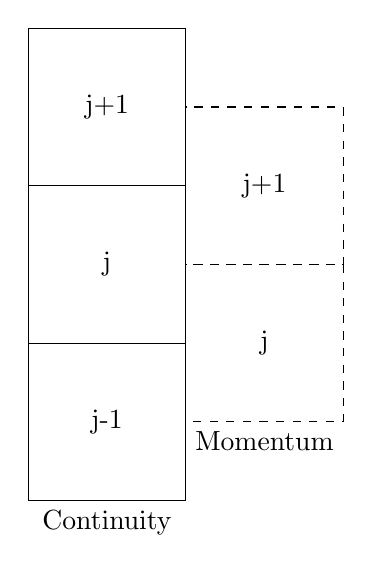
\begin{tikzpicture}
\draw (-2,-3) rectangle +(2,2);
\node[anchor=center] at (-1,-2) {j-1};
\draw (-2,-1) rectangle +(2,2);
\node[anchor=center] at (-1, 0) {j};
\draw (-2, 1) rectangle +(2,2);
\node[anchor=center] at (-1, 2) {j+1};
\draw[dashed] (-0,-2) rectangle +(2,2);
\node[anchor=center] at (1, -1) {j};
\draw[dashed] (-0, 0) rectangle +(2,2);
\node[anchor=center] at (1, 1) {j+1};
\node[anchor=north] at (-1, -3) {Continuity};
\node[anchor=north] at (1, -2) {Momentum};
\end{tikzpicture}
\caption{Illustration of indexing scheme.}
\label{fig:vertical_pipe_with_cells}
\end{figure}

Recalling the staggered mesh from \sect{sect:geometry}, the six scalar conservation laws, \eqref{eqn:conservation_of_ncg} -- \eqref{eqn:con_energy_liq}, are each integrated over the continuity volumes.
The assumption in these integrals is that the value of the conserved quantities and all thermodynamically-related variables are a constant, average value within a given continuity volume.
\fig{fig:constant_value} shows a graphical representation of this idea for a generic function $f(x)$ over several spatial continuity volumes. 

\begin{figure}[ht!]
\centering
\tikzsetnextfilename{images/constant_value_pdf}
\begin{tikzpicture}
\draw [->, thick] (-5,0) -- (6,0);
\draw [->, thick] (-5,0) -- (-5,4);
\draw (-4,1) -- (-1,1);
\draw (-1,2) -- (2,2);
\draw (2,3) -- (5,3);
\draw (-5.5,3) node {$f(x)$};
\draw [dashed] (-4,1) -- (-4,0);
\draw [dashed] (-1,2) -- (-1,0);
\draw [dashed] (2,3) -- (2,0);
\draw [dashed] (5,3) -- (5,0);
\foreach \x / \xtext in {-2.5/x_{j-1},-1/x_{j-\onehalf},0.5/x_j,2/x_{j+\onehalf},3.5/x_{j+1}}
	\draw [thick] (\x,-2pt) -- (\x,0pt) node [anchor=north] {$\xtext$};
\end{tikzpicture}
\caption{Constant variable values within computational volumes.}
\label{fig:constant_value}
\end{figure}

Within a subchannel, a given continuity volume of length $\Delta x $ has a constant cross-sectional area, $A_{c}$, over its length.
The cross-sectional area of the boundary between two continuity volumes is given by the cross-sectional area of the momentum path at that boundary, $A_{m}$.

\begin{figure}[ht!]
\centering
\tikzsetnextfilename{images/isoparametric_volume_pdf}
\begin{tikzpicture}
\draw [dotted] (2,0) arc (0:180:2 and 1);
\draw (-2,0) arc (180:360:2 and 1);
\draw [dashed] (0,4) circle (2 and 1);
%\filldraw [black] (0,4) circle (2pt);
\draw [pattern=dots] (0,8) circle (2 and 1);
\draw (-2,0) -- (-2,8);
\draw (2,0) -- (2,8);
\draw [<->] (2.75,0) -- (2.75,8);
\draw (2.5,0) -- (3,0);
\draw (2.5,8) -- (3,8);
\draw (3.25,4) node {$\Delta x_j$};
\filldraw [gray!10] (0,8) circle (0.5);
\draw (0,8) node {$A_{C,j}$};
\foreach \y/\ytext in {0/$x_{j-\frac{1}{2}}$,4/$x_j$,8/$x_{j+\frac{1}{2}}$}
	\draw (-2.25,\y) node [anchor=east] {\ytext};
\end{tikzpicture}
\caption{Single continuity volume, $V_{j}$, over which the conservation equations are integrated.}
\label{fig:single_volume}
\end{figure}

For illustrative purposes \eqref{eqn:conservation_of_liq} will be integrated over a simplified volume, $V_j$, consisting of singly connected axial flow as shown in \fig{fig:single_volume}.
This volume integrated equation is given by \eqref{eqn:spatially_discrete_liq_m_con}.
The same general procedure is used for the other five scalar conservation equations.

\begin{IEEEeqnarray}{lcl}
\int_{V_j}\frac{\partial \left(\alpha_l \rho_l \right)}{\partial t } & + & \nabla \cdot \left( \alpha_l \rho_l u_l \right) \mathrm{d}V = \int_{V_j} \left(-(1-\eta)\dot{\Gamma}^{'''} - \dot{\Upsilon}^{'''} + \dot{s}^{'''}_{m,l}\right) \mathrm{d}V \nonumber \\
V_j \frac{\partial \left(\alpha_{l,j} \rho_{l,j} \right)}{\partial t } & = & -\int_{V_j}\nabla \cdot \left( \alpha_l \rho_l u_l \right) \mathrm{d}V -(1-\eta_j)\dot{\Gamma}_j - \dot{\Upsilon}_j + \dot{s}_{m,l,j} \nonumber \\
V_j \frac{\partial \left(\alpha_{l,j} \rho_{l,j} \right)}{\partial t } & = & -\left[\alpha_l \rho_l u_l A_{m}\right]_{x_{j-\onehalf}}^{x_{j+\onehalf}} -(1-\eta_j)\dot{\Gamma}_j - \dot{\Upsilon}_j + \dot{s}_{m,l,j} \nonumber \\
\label{eqn:spatially_discrete_liq_m_con}
V_j \frac{\partial \left(\alpha_{l,j} \rho_{l,j} \right)}{\partial t } & = & -\left( \don{\alpha_l \rho_l}_{\text{d},j+\onehalf} u_{l,j+\onehalf} A_{m,j+\onehalf} - \don{\alpha_l \rho_l}_{\text{d},j-\onehalf} u_{l,j - \onehalf} A_{m,j - \onehalf}\right) \nonumber \\
& & -(1-\eta)\dot{\Gamma}_j - \dot{\Upsilon}_j + \dot{s}_{m,l,j}
\end{IEEEeqnarray}

For the mass-flux terms evaluated on the continuity volume edge, the advected quantity is evaluated using a 1st order upwind method \cite{Tannehill1997}.
The velocity and cross-sectional area utilized in the continuity flux terms, $u_{j \pm \onehalf}$ and $A_{m,j \pm \onehalf}$, have the values defined in the momentum path that aligns with the boundary of continuity volumes.
The sign of the velocity at the volume boundary determines the value of the donored quantity, $\don{a}_{\text{d},j \pm \onehalf}$.
A more generic formulation for this scheme is given by \eqref{eqn:upwind_donoring}.
The superscripts, $b$ and $c$, denote the discrete points in time at which the variables are evaluated.
The particular time superscripts in \eqref{eqn:upwind_donoring} are for illustrative purposes and are not fixed.

\begin{equation}
\label{eqn:upwind_donoring}
\don{a^{b}}^{c}_{\text{d}, j - \onehalf} = \begin{cases} a^{b}_{j-1} &  u^{c}_{j - \onehalf} \geq 0 \\ a^{b}_{j} & u^{c}_{j - \onehalf} < 0 \end{cases}
\end{equation}

The three momentum conservation equations, \eqref{eqn:con_mom_liq} -- \eqref{eqn:con_mom_ent}, are integrated over their momentum flow path.
The cross-sectional area for a momentum path, $A_{m}$, can be defined independently of the two cross-sectional areas of the adjoining continuity volumes.
The momentum flux terms, \eqref{eqn:momentum_flux_terms}, are treated similarly to the flux terms in the continuity equations.

\begin{equation}
\label{eqn:momentum_flux_terms}
-\left[\don{\alpha_l \rho_l u_l}_{\text{d}} \ave{u_{l}}_{\text{a}} \tilde{A}\right]_{x_{j }}^{x_{j + 1}}
\end{equation}

There are two primary differences.
First, the area in the flux term, $\tilde{A}$, is taken as the minimum of two areas from the adjoining momentum flow paths, \eqref{eqn:area_def}.

\begin{equation}
\label{eqn:area_def}
\tilde{A}_{j} = \min\left(A_{m,j - \onehalf}, A_{m,j+\onehalf}\right)
\end{equation}

Second, the phasic velocity that is used to determine the donored quantities is the arithmetic mean of the velocities from the two adjacent momentum flow paths, \eqref{eqn:average_advecting_vel}.

\begin{equation}
\label{eqn:average_advecting_vel}
\ave{u}_{\text{a},\phi, j} = \frac{u_{\phi, j - \onehalf} + u_{\phi, j+ \onehalf}}{2}
\end{equation}

The ordering of the governing equations within a given continuity volumes is as follows:

\begin{enumerate}
\item{Conservation of the \ncg{} field mass.}
\item{Conservation of the continuous liquid field mass.}
\item{Conservation of the gaseous phase energy.}
\item{Conservation of the liquid phase energy.}
\item{Conservation of the entrained liquid field mass.}
\item{Conservation of the vapor field mass.}
\end{enumerate}

The conservation of momentum equations within a given momentum flow path are ordered as follows:

\begin{enumerate}
\item{Conservation of the continuous liquid field momentum.}
\item{Conservation of the gaseous phase momentum.}
\item{Conservation of the entrained liquid field momentum.}
\end{enumerate}

%-------------------------------------------------------------------------------
%-------------------------------------------------------------------------------
%-------------------------------------------------------------------------------
\subsection{Temporal Approximations}
\label{subsect:temporal_approx}

Once the governing conservation equations have been spatially discretized utilizing the method outlined above, the temporal derivatives need to be approximated numerically.
The continuous conservation equations, \eqref{eqn:conservation_equations}, are now a spatially-discrete, temporally-continuous set of equations given by \eqref{eqn:temporal_semi_discrete}, where $\vec{E}$ now represents the spatially discrete approximation of $\vec{e}$.

\begin{equation}
\label{eqn:temporal_semi_discrete}
\frac{\partial \,\vec{y} }{\partial t} = \vec{E}(\vec{y}(t))
\end{equation}

Given that there are nine conservation equations, nine independent parameters need to be chosen.
The choice of the nine variables that will be solved for is another distinguishing characteristic of safety analysis software.
This work uses the following set of nine independent variables \eqref{eqn:independentVariables}.

\begin{equation}
\label{eqn:independentVariables}
\vec{x} = [\alpha_{g}P_{n}, \alpha_g, \alpha_g h_v, (1 - \alpha_g) h_l, \alpha_e, P, \dot{m}_g, \dot{m}_l, \dot{m}_e]^{T}
\end{equation}

The definition of the conserved momentum quantity for a given phase, $\dot{m}_{\phi}$, is given by \eqref{eqn:mom_dot}.

\begin{equation}
\label{eqn:mom_dot}
\dot{m}_{\phi} = \ave{\alpha_{\phi} \rho_{\phi}}_{\text{a}} u_{\phi} A_{m}
\end{equation}

The averaging operator $\ave{a}_{\text{a}}$ provides the average of a quantity from the two adjoining continuity volumes, \eqref{eqn:average_val}.

\begin{equation}
\label{eqn:average_val}
\ave{a}_{\text{a},j + \onehalf} = \frac{a_{j} + a_{j+1}}{2}
\end{equation}

The use of the momenta and the product of phasic volume fractions and phasic enthalpies, such as $\alpha_g h_v$, as independent parameters represents a unique choice.
However, these independent parameters are not the only option for safety analysis software.
Other software, such as TRACE and \relap53d{}, use variants of these parameters.
These variations include the use of velocities instead of momenta, and temperatures or internal energies instead of enthalpies \cite{RELAP, TRACE}.

A distinguishing feature of the numerical method in \cobra{} is its treatment of the temporal derivative for the conservation of momentum.
In the work that follows the temporal derivative of the conserved momentum equations is directly discretized, which is known as the conservative form.
The other option, the non-conservative form, expands the temporal derivative analytically via the chain rule, \eqref{eqn:non_conservative}, and these equations are then temporally discretized.

\begin{equation}
\label{eqn:non_conservative}
\frac{\partial \alpha_{\phi} \rho_{\phi} u_{\phi}}{\partial t} = \alpha_{\phi} \rho_{\phi} \frac{\partial u_{\phi}}{\partial t} + u_{\phi} \frac{\partial \alpha_{\phi} \rho_{\phi}}{\partial t}
\end{equation}

In this work the temporal derivative is approximated by a one-step difference scheme where the continuous time variables are now evaluated at discrete points, $t^0, t^1, \ldots, t^{N_{t}}$.
The notations $t^0$ and $t^{N_{t}}$ represent the initial and final time, respectively.
The term ``one-step" refers to the fact that the temporal derivative involves only two consecutive points in time.
The integral over a time interval, $\dt{} = t^{n+1} - t^{n}$, is show in \eqref{eqn:simple_partial_t}.

\begin{IEEEeqnarray}{rcl}
\int^{t^{n+1}}_{t^n}\frac{\partial \vec{y}(\vec{x})}{\partial t}\mathrm{d}\tau & = & \int^{t^{n+1}}_{t^n}\vec{E}(\vec{y}(\vec{x}))\mathrm{d}\tau \nonumber \\
\vec{y}(\vec{x}^{n+1}) - \vec{y}(\vec{x}^{n}) & = & \int_{t^{n+1}}^{t^n}\vec{E}(\vec{y}(\vec{x}))\mathrm{d}\tau \nonumber  \\
\vec{y}(\vec{x}^{n+1}) - \vec{y}(\vec{x}^{n}) & = & \Delta t \vec{E}(\vec{y}(\vec{x}^{*})) \nonumber  \\
\label{eqn:simple_partial_t}
\frac{\vec{y}(\vec{x}^{n+1}) - \vec{y}(\vec{x}^{n})}{\Delta t} & = & \vec{E}(\vec{y}(\vec{x}^{*}))
\end{IEEEeqnarray}

The choice of how to approximate the temporal integral of the sources and sinks of the system, $\vec{E}(\vec{y}(\vec{x}^{*}))$, hereafter referred to as $\vec{E}^{*}$, is a factor that defines the eventual solution algorithm.
There are two subcategories for solving this one-step temporal-integration problem, single-stage and multi-stage \cite{Stewart1981,LeVeque2007}.
\alg{alg:single_stage_temporal} shows how a multi-stage temporal integration scheme would work.

\begin{algo}[ht!]
\setlength{\baselineskip}{0.625\baselineskip}
\begin{algorithmic}[1]
\Require $\vec{y}^{0}$ and $t^{0}$
\Set $n = 0$
\Loop \; Transient Loop
    \State $t^{n+1} : = t^{n} + \Delta t$
    \For{$s = 1 \to N_{s}$} \; Stage Loop
		\BlackBox Solve $\displaystyle \frac{\vec{y}^{s} - \vec{y}^{n}}{\Delta t} =  \vec{E}^{*,s}$ for $\vec{y}^{s}$.
	\EndFor
	\State $n = n + 1$
\EndLoop
\end{algorithmic}
\caption{Multi-stage temporal integration scheme.}
\label{alg:single_stage_temporal}
\end{algo}

The final-stage conserved variables will be the new-time variables, $\vec{y}^{N_{s}} = \vec{y}^{n+1}$. 
At each stage the choice of how to approximate the driving function, $\vec{E}^{*,s}$, can change in both its functional dependence upon the stage values of $\vec{y}^{s}$ and in which components of $\vec{E}^{*}$ are included.
By excluding certain portions of $\vec{E}^{*}$ at certain stages, a time-splitting algorithm is developed.
Time-splitting algorithms are also known as operator-splitting algorithms. 
By changing the functional dependencies of terms within $\vec{E}^{*}$ at different stages, predictor-corrector methods, also called stabilizing correction methods, are generated. 
A single-stage method is the degenerate multi-stage case of $N_{s} = 1$.

For this work the conserved quantities within a continuity volume (e.g., $\alpha_g \rho_g$, $\left(1-\alpha_g\right)\rho_l h_l$) are nonlinear functions of the chosen independent parameters, \eqref{eqn:nonlinear_functions}, regardless of the approximation chosen for $\vec{E}^{*}$.

\begin{equation}
\label{eqn:nonlinear_functions}
\vec{y}^{n+1} = \vec{y}(\vec{x}^{n+1})
\end{equation}

This nonlinearity necessitates the use of a nonlinear solver at every timestep.
Any dependence of $\vec{E}^{*}$ on the new-time parameters creates additional nonlinearities.
The discrete formulation, \eqref{eqn:simple_partial_t}, can be expressed as a nonlinear residual of $\vec{x}^{n+1}$ by \eqref{eqn:nonlinear_residuals}.

\begin{equation}
\label{eqn:nonlinear_residuals}
\vec{F}(\vec{x}^{n+1}) = \vec{y}(\vec{x}^{n+1}) - \vec{y}(\vec{x}^n) -\Delta t \vec{E}^{*}
\end{equation}

The temporal integration method used has an associated temporal accuracy that depends upon the approximation of $\vec{E}^{*}$ and the number of stages. 
The temporal accuracy is a way of quantifying the behavior of the solution as the timestep is reduced.
Order of accuracy estimates for temporal integration techniques are proportionality statements between the numerical error and a power of the timestep, $\mathcal{O}(\dt{}^{p})$ \cite{LeVeque2007}. 
However, it has been shown that if the nonlinear problem, \eqref{eqn:nonlinear_residuals}, is not solved at every timestep, the temporal accuracy of a method can be degraded \cite{Knoll2001, Mahaffy1993}.

%-------------------------------------------------------------------------------
%-------------------------------------------------------------------------------
%-------------------------------------------------------------------------------
\subsection{Nonlinear Approximations}
\label{subsect:nonlinear_approximations}

The method used to solve \eqref{eqn:nonlinear_residuals} for $\vec{x}^{n+1}$ in this work is Newton's method \cite{Deuflhard2004, Dennis1996}.
The nonlinear residual is a function of the new-time unknowns, $\vec{x}^{n+1}$.
Newton's method is an iterative procedure to obtain $\vec{x}^{n+1,k}$ such that $\vec{F}(\vec{x}^{n+1,k}) = 0$.
Since Newton's method is an iterative procedure for obtaining the correct new-time variables, two superscripts are required.
The nonlinear iterate superscript will be $k$.
Successive linearization of the nonlinear problem, \eqref{eqn:newton_taylor}, generates an iterative solution method.

\begin{equation}
\label{eqn:newton_taylor}
0 = \vec{F}(\vec{x}^{n+1,k}+\vec{\delta x}^k) \approx \vec{F}(\vec{x}^{n+1,k}) + \vec{J}(\vec{x}^{n+1,k}) \cdot \vec{\delta x}^k
\end{equation}

The algorithm is then one of finding successive updates, $\vec{\delta x}^k = \vec{x}^{n+1,k+1} - \vec{x}^{n+1,k}$, by solving \eqref{eqn:newton}.

\begin{equation}
\label{eqn:newton}
\vec{J}(\vec{x}^{n+1,k})\cdot \vec{\delta x}^k = -\vec{F}(\vec{x}^{n+1,k})
\end{equation} 

Since the system of nonlinear equations being solved represents a transient simulation, the iterations at each timestep start with an initial guess for the new-time variables that is equal to the old-time variables, $\vec{x}^{n+1,0} = \vec{x}^{n}$.
The underlying assumption of this initial value is that the independent parameters will not change greatly over a timestep, and the old-time variables will provide an initial vector that is within the radius of convergence of Newton's method.
\alg{alg:local_newton} provides an overview of a transient simulation using a Newton's method for a single-stage temporal integration scheme.
The algorithm generalizes to a multi-stage temporal integration method by enclosing the Newton loop within a stage loop.

\begin{algo}[ht!]
\setlength{\baselineskip}{0.625\baselineskip}
\begin{algorithmic}[1]
\Require $\vec{x}^{0}$ and $t^{0}$
\Set $n = 0$
\Loop \; Transient Loop
    \Set $t^{n+1} = t^{n} + \dt{}$
    \Set $k = 0$
    \Set $\vec{x}^{n+1,k} = \vec{x}^{n}$
    \Loop \; Newton Loop
		\Calculate $\vec{F}(\vec{x}^{n+1,k})$ and $\vec{J}(\vec{x}^{n+1,k})$
		\Calculate $\vec{\delta x}^k = - \vec{J}^{-1}\cdot\vec{F}$
		\Calculate $\vec{x}^{n+1,k+1} = \vec{x}^{n+1, k} + \vec{\delta x}^{k}$
		\Set $k \pluseq 1$
		\BlackBox Loop Termination Criteria
	\EndLoop
	\Set $n \pluseq 1$
\EndLoop
\end{algorithmic}
\caption{Local Newton's method for single-stage temporal integration.}
\label{alg:local_newton}
\end{algo}

In \alg{alg:local_newton}, there is a black box step, the calculation of the loop termination criteria.
In multi-stage temporal integration methods the loop termination criteria may vary between stages. 
In the case where the loop is terminated after only a single iterate the resultant method is labeled a single-shot linearization.

%-------------------------------------------------------------------------------
%-------------------------------------------------------------------------------
%-------------------------------------------------------------------------------
\section{Solution Methods}
\label{sect:solution_techniques}

\sect{sect:numeric_approximation} provided a framework for characterizing the different solution methods used in thermal-hydraulic safety codes. 
Each method can be defined by the manner in which the temporal integration is carried out and the manner in which the nonlinearities are resolved.
The methods described below form the core of available techniques that have been developed for two-phase safety analysis codes. 
While each of the following methods may have many subtly varying algorithmic implementations that have appeared in safety analysis software, the algorithms detailed below are general enough to encompass these variants.

%-------------------------------------------------------------------------------
%-------------------------------------------------------------------------------
%-------------------------------------------------------------------------------
\subsection{Fully Explicit Method}
\label{subsect:numerics_explicit}
The least computationally expensive method on a per timestep basis for temporally integrating \eqref{eqn:simple_partial_t} is a single-stage, fully explicit method.
In the fully explicit method, the driving function is approximated as $\vec{E}(\vec{x}^n)$.
The nonlinear vector notation formulation for this method is given by \eqref{eqn:explicit}.

\begin{equation}
\label{eqn:explicit}
\vec{F}(\vec{x}^{n+1}) = \vec{y}(\vec{x}^{n+1}) - \vec{y}^{n} - \Delta t \vec{E}(\vec{y}(\vec{x}^{n}))
\end{equation}

The algorithmic implementation is shown in \alg{algo:explicit}.
Given the choice of independent parameters in this work, there are nonlinearities present \eqref{eqn:explicit}.

\begin{algo}[ht!]
\setlength{\baselineskip}{0.625\baselineskip}
\begin{algorithmic}[1]
\Require $\vec{x}^{0}$ and $t^{0}$
\Set $n = 0$
\Loop \; Take a Timestep
    \State $t^{n+1} : = t^{n} + \Delta t$
    \Calculate $\vec{F}(\vec{x}^n)$ and $\vec{J}(\vec{x}^n)$
    \Calculate $\vec{\delta x} = -\vec{J}^{-1}\vec{F}$
    \Calculate $\vec{x}^{n+1} = \vec{x}^{n} + \vec{\delta x}$ 
\EndLoop{\;$n \pluseq n+1$}
\end{algorithmic}
\caption{Single-stage, fully explicit, single-shot linearization method.}
\label{algo:explicit}
\end{algo}

While this particular method is the least computationally expensive on a per timestep basis of those discussed, it has a severe weakness.
That weakness is the Courant-Friedrichs-Lewy (CFL) limit imposed upon the timestep size, $\dt{}$.
The CFL limit is a relationship between the spatial and temporal discretization and the characteristic velocities of information propagation in the problem of interest \cite{LeVeque2007, Tannehill1997}.
For the case of \eqref{eqn:explicit}, the CFL limit is given in \eqref{eqn:cfl_explicit}.

\begin{equation}
\label{eqn:cfl_explicit}
\dt{}_i \lesssim \frac{\dx{}_i}{|u_{\phi,i}|+|c_i|}
\end{equation}

In \eqref{eqn:cfl_explicit}, $c_i$ and $u_i$ are the speed of sound and the magnitude of a given phasic velocity, respectively, at a given location within the domain.
These two velocities, for most applications of interest, can be of drastically different magnitude.
For example, in single phase gaseous flow, the ratio of the local phasic velocity to the speed of sound is typically much less than one ($\approx 0.01$) for problems of interest.
Using the local fluid conditions, $\dt{}_i$ is calculated at every point within the domain, $\Omega$.
The $\dt{}$ chosen for the $t^{n} \rightarrow t^{n+1}$ timestep is the most restrictive calculated value over the domain, \eqref{eqn:global_cfl}.

\begin{equation}
\label{eqn:global_cfl}
\dt{} = \min_{i \in \Omega} \dt{}_i
\end{equation}

Since the CFL limit is based upon the local speed of sound it is referred to as the sonic Courant limit.
While the explicit method may provide the lowest computational cost on a per-timestep basis, the number of timesteps required for a given problem may be much greater than the following methods due to this restrictive CFL limitation.
This limitation of the explicit method prompted the development of alternative methods that were capable of exceeding this Courant limit.

%-------------------------------------------------------------------------------
%-------------------------------------------------------------------------------
%-------------------------------------------------------------------------------
\subsection{Fully Implicit Method}
\label{subsect:numerics_fully_implicit}
One alternative method for integrating \eqref{eqn:temporal_semi_discrete} is to use a fully implicit discretization of $\vec{E}^{*}$ \cite{Frepoli2003, Barre1990}.
The fully implicit method temporally approximates $\vec{E}^{*}$ as a function  of new-time parameters only, \eqref{eqn:implicit}.

\begin{equation}
\label{eqn:implicit}
\vec{F}(\vec{x}^{n+1}) = \vec{y}(\vec{x}^{n+1}) - \vec{y}^{n} - \Delta t \vec{E}(\vec{y}(\vec{x}^{n+1}))
\end{equation}

This method has the advantage of not being limited by a CFL number.
While this allows for greatly increased timestep sizes, the numerical scheme introduces nonphysical diffusion into the solution \cite{Mahaffy1993}.
Additionally, the solution of \eqref{eqn:implicit} is the most computationally expensive on a per timestep basis of the methods considered.
This computational expense comes from the full inter-volume coupling of the Jacobian matrix during the nonlinear iterations.
The computational implementation of a fully implicit method is presented in \alg{algo:implicit}.
The black-box step in \alg{algo:implicit} will be discussed in \sect{subsect:nlnCobraAlgo}.

\begin{algo}[ht!]
\setlength{\baselineskip}{0.625\baselineskip}
\begin{algorithmic}[1]
\Require $\vec{x}^{0}$ and $t^{0}$
\Set $n = 0$
\Loop \; Transient Loop
    \Set $t^{n+1} : = t^{n} + \Delta t$
    \Set $k = 0$
    \Set $\vec{x}^{k} = \vec{x}^{n}$
    \Loop \; Newton Loop
		\Calculate $\vec{F}(\vec{x}^{k})$ and $\vec{J}(\vec{x}^{k})$
		\Calculate $\vec{\delta x}^k = - \vec{J}^{-1}\cdot\vec{F}$
		\Calculate $\vec{x}^{k+1} = \vec{x}^{k} + \vec{\delta x}^{k}$
		\Set $k \pluseq 1$
		\BlackBox Loop Termination Criteria
	\EndLoop	
	\Set $n \pluseq 1$
\EndLoop
\end{algorithmic}
\caption{Fully implicit method.}
\label{algo:implicit}
\end{algo}

%-------------------------------------------------------------------------------
%-------------------------------------------------------------------------------
%-------------------------------------------------------------------------------
\subsection{Semi-Implicit Method}
\label{subsect:semi_implicit}

Another alternative method for integrating \eqref{eqn:temporal_semi_discrete} is the semi-implicit method.
It was developed to overcome the sonic Courant limitations of the explicit method while avoiding both the high computational cost and excessive diffusivity of the fully implicit method \cite{Liles1978}.
The two distinguishing characteristics of the semi-implicit method are the use of new-time variables in the evaluation of the pressure gradient in the momentum conservation equations and in the advecting velocities in the mass and energy equations. 
The implicit evaluation of the pressure gradient in the momentum equations is what leads to a CFL limit known as the material Courant limit.
Similar to the sonic Courant limit discussed in \sect{subsect:numerics_explicit}, the material Courant limit dictates the largest $\Delta t$ that can be achieved while maintaining a stable solution algorithm.
In this method the Courant limit is given by \eqref{eqn:si_cfl}.

\begin{equation}
\label{eqn:si_cfl}
\dt{}_i \lesssim \frac{\dx{}_i}{|u_{\phi,i}|}
\end{equation}

The characteristic velocity used in the calculation of the Courant limit is based on the phasic velocity only.
This allows for larger, but still limited, timestep sizes than the fully explicit method.
The limit on timestep size is due to the explicit evaluation of the donored quantities in the flux terms in the conservation equations.
As stated, the flux of mass and energy include new-time velocities, $u^{n+1}_{\phi}$.
Since this work uses momenta, $\dot{m}_{\phi}$, as independent parameters, these velocities are derived quantities, whose functional form is given in \eqref{eqn:si_vel}.
The $\ave{\alpha_{\phi} \rho_{\phi}}^{n}_{\text{a}}$ represents the arithmetic average of macroscopic densities from adjoining continuity volumes.
The averaging operator $\ave{a}^{n}_{\text{a}}$ is an extension of \eqref{eqn:upwind_donoring}.
There is a mismatch between the averaged macroscopic density and the momentum in \eqref{eqn:si_vel}.
This mismatch will be discussed in more detail in \sect{subsect:nlnPhaseTransition}.

\begin{equation}
\label{eqn:si_vel}
u^{n+1}_{\phi, j \pm \onehalf} = \frac{\dot{m}^{n+1}_{\phi, j \pm \onehalf}}{A_{m, j \pm \onehalf} \ave{\alpha_{\phi} \rho_{\phi}}^{n}_{\text{a}, j \pm \onehalf}} 
\end{equation}

\alg{alg:si_legacy} shows the algorithm for solving the semi-implicit method.

\begin{algo}[ht!]
\setlength{\baselineskip}{0.625\baselineskip}
\begin{algorithmic}[1]
\Require $\vec{x}^{0}$ and $t^{0}$
\Set $n = 0$
\Loop \; Transient Loop
    \Set $t^{n+1} : = t^{n} + \Delta t$
	\Calculate $\vec{F}(\vec{x}^{n})$ and $\vec{J}(\vec{x}^{n})$
	\Calculate $\vec{\delta x} = - \vec{J}^{-1}\cdot\vec{F}$
	\Calculate $\vec{x}^{n+1} = \vec{x}^{n} + \vec{\delta x}$
	\Set $n \pluseq 1$
\EndLoop
\end{algorithmic}
\caption{Semi-implicit method.}
\label{alg:si_legacy}
\end{algo}

%-------------------------------------------------------------------------------
%-------------------------------------------------------------------------------
%-------------------------------------------------------------------------------
\subsection{Stability-Enhancing Two-Step Method} 
\label{subsect:numerics_sets}
In order to overcome the material Courant limit placed upon simulations by the semi-implicit method, the Stability Enhancing Two-Step (SETS) method was developed \cite{Mahaffy1982}.
While not as stable as the fully implicit method, the SETS method allows for timesteps to exceed the material Courant limit.
It overcomes the material Courant limit by taking a multi-stage approach to the temporal integration.
While there are variants of the SETS method \cite{TRACE}, \alg{alg:sets} reflects the original publication.
The outline below uses velocities as independent parameters, not momenta.

There are three stages in the original SETS method.
Stage one is a single-shot linearized solution of the momentum equations where only the velocity terms in the momentum equations of $\vec{E}^{*}$ are evaluated implicitly.
This first stage only involves the solution of the momentum equations; the mass and energy equations are not solved during this step.
The lack of implicit dependence upon any continuity variables allows for coupling only between momentum flow paths.
This step results in predicted $u^{*}_{\phi}$ phasic velocities.

In stage two, the momentum and continuity equations are solved using a traditional semi-implicit scheme with two exceptions.
The first is that the momentum flux terms are evaluated using the stage-one predicted velocities as the advecting velocities instead of explicitly evaluating them.
The second is that the nonlinearities in the momentum equations, arising from interfacial and wall drag, are subject to a single-shot linearization.
The single-shot nature of the momentum equations allows for the reduction of the system into coupled continuity volumes as in the semi-implicit method.
The nonlinear continuity equations are then solved via Newton's method.
Stated another way, the Jacobians for the momentum equations are fixed at their first Newton iterate value, while the Jacobians for the mass and energy equations are updated at each iterate.

In the third stage the mass and energy equations are solved such that all continuity variables are implicitly evaluated but the velocities are from stage two.
These velocities, $\vec{u}^{2}$, are the only results from stage two that are used in stage three. 
The resulting system of coupled continuity equations is then solved.
This final stage allows timestep sizes that exceed the material Courant limit.
For each stage the residual and Jacobian matrix will be denoted by $\vec{F}^{s}$ and $\vec{J}^{s}$, with $s = 1 \to 3$.

\begin{algo}[ht!]
\setlength{\baselineskip}{0.625\baselineskip}
\begin{algorithmic}[1]
\Require $\vec{x}^{0}$ and $t^{0}$
\Set $n = 0$
\Loop \; Transient Loop
    \Set $t^{n+1} : = t^{n} + \Delta t$
	\Calculate $\vec{F}^{1}$ and $\vec{J}^{1}$
	\Calculate $\vec{u}^{*}$ from $\vec{\delta u}^{*} = -\left[\vec{J}^{1}\right]^{-1} \vec{F}^{1}$
	\Loop \; Newton Loop
		\Calculate $\vec{F}^{2}$ and $\vec{J}^{2}$
		\Calculate $\vec{\delta x} = - \left[\vec{J}^{2}\right]^{-1} \vec{F}^{2}$
		\Calculate $\vec{x}^{n+1} = \vec{x}^{n} + \vec{\delta x}$
		\BlackBox Loop Termination Criteria
	\EndLoop
	\Calculate $\vec{x}^{n+1}$ from $\vec{F}^{3}$.
	\Set $n \pluseq 1$
\EndLoop
\end{algorithmic}
\caption{SETS method.}
\label{alg:sets}
\end{algo}

This algorithm was designed to allow existing software utilizing the semi-implicit method to be embedded within a larger framework.
The black-box loop termination criteria is a choice that varies with implementation.
The TRACE code uses an $\mathcal{L}_{\infty}$ norm of the unscaled Newton updates for the continuity variables to determine convergence.

%-------------------------------------------------------------------------------
%-------------------------------------------------------------------------------
%-------------------------------------------------------------------------------
\subsection{Nearly-Implicit Method}
\label{subsect:numerics_nearly_implicit}
Another possible method used to overcome the material Courant limit without incurring the same computational cost as the fully implicit method is the Nearly-implicit method \cite{Trapp1986, RELAP}.
The Nearly-Implicit method is a multistage temporal integration scheme.
In the first stage the approximation  of $\vec{E}^{*}$ is one in which the mass and energy terms are implicit except for the donored values in the flux terms. 
In addition, the the chain rule is applied to the continuous temporal derivatives, resulting in mass equations similar to \eqref{eqn:ni_dt}.
The energy temporal derivatives are similarly expanded.

\begin{equation}
\label{eqn:ni_dt}
\frac{\partial \alpha_{\phi} \rho_{\phi}}{\partial t} = \alpha_{\phi} \frac{\partial \rho_{\phi}}{\partial t} + \rho_{\phi} \frac{\partial \alpha_{\phi}}{\partial t}
\end{equation}

The temporal discretization of \eqref{eqn:ni_dt} is given by \eqref{eqn:ni_dis_dt}.

\begin{equation}
\label{eqn:ni_dis_dt}
\alpha_{\phi} \frac{\partial \rho_{\phi}}{\partial t} + \rho_{\phi} \frac{\partial \alpha_{\phi}}{\partial t} = \alpha^{n}_{\phi} \frac{ \rho^{n+1}_{\phi} - \rho^{n}_{\phi}}{\dt{}} + \rho^{n}_{\phi} \frac{\alpha^{n+1}_{\phi} - \alpha^{n}_{\phi} }{\dt}
\end{equation}

The momentum equations are implicit in their momentum flux, pressure, and interfacial exchange terms.

The Nearly-Implicit method is a three-stage solution process.
The first stage is similar to the semi-implicit method.
However, as opposed to the semi-implicit method where the momentum variables are eliminated from the equations being solved, the Nearly-Implicit method uses the mass and energy equations to eliminate the pressure terms from the momentum equations.
The resulting matrix is a linear system of coupled velocities.
The stage-one velocities are taken to be the new-time velocities.
Once the stage-one velocities are obtained, the corresponding stage-one continuity variables are obtained analogously to the new-time momentum in the semi-implicit method.
Stage one is a single-shot linearization.
In the second stage, only the continuity equations are solved and they are in conservative form.
The interfacial exchange terms in the mass and energy equations are evaluated using the stage-one continuity variables.
The resulting system of equations is linear in the conserved quantities.
This linear system is solved for the conserved quantities.
In stage three, the nonlinear relation between the conserved quantities and the independent parameters is then approximated via a single-shot linearization of the equations of state.
\alg{alg:ni} shows the three-stage process.

\begin{algo}[ht!]
\setlength{\baselineskip}{0.625\baselineskip}
\begin{algorithmic}[1]
\Require $\vec{x}^{0}$ and $t^{0}$
\Set $n = 0$
\Loop \; Transient Loop
    \Set $t^{n+1} : = t^{n} + \Delta t$
	\Calculate $\vec{F}^{1}$ and $\vec{J}^{1}$
	\Calculate $\vec{x}^{*}$ and $\vec{u}^{n+1}$ from $\vec{\delta x}^{*} = -\left[\vec{J}^{1}\right]^{-1} \vec{F}^{1}$
	\Calculate $\vec{F}^{2}$
	\Calculate $\vec{x}^{**}$ from $\vec{F}^{2}$
	\Calculate $\vec{x}^{n+1}$ from $\vec{F}^{3}$.
	\Set $n \pluseq 1$
\EndLoop
\end{algorithmic}
\caption{Nearly-Implicit method}
\label{alg:ni}
\end{algo}

%-------------------------------------------------------------------------------
%-------------------------------------------------------------------------------
%-------------------------------------------------------------------------------
\section{Domain Coupling}
\label{sect:code_coupling}

\cobra{} possesses models of the physics necessary to simulate the complicated in-core flow patterns and heat transfer encountered during a postulated LOCA.
However, it lacks the detailed models for NPP components (pumps, valves, accumulators, pressurizers) that are traditionally available from system analysis codes.
When modeling full NPP transients, it is advantageous to use sub-channel software for the core and system analysis software for the rest of the NPP.
The combination of different specialized software is a common practice.
This coupling of capabilities can be accomplished in two ways: the two pieces of software can be merged or they can be coupled via data exchange.
Examples of the first method are MARS \cite{Jeong2008}, COBRA/TRAC \cite{Thurgood1983c}, and TRACE \cite{TRACE}.
Coupling software via data exchange is a more common option \cite{Makihara2003, Aumiller2002, Aumiller2001, Avramova2006, Weaver2002, Rodriguez2002}, and it will be discussed first.

When coupling via data exchange, the use of explicit coupling can lead to a sonic Courant limit imposed at the boundary of the two coupled systems \cite{Ragusa2009, Aumiller2001}.
To circumvent the sonic Courant limit, a semi-implicit method for the coupling of software via data exchange has been developed for thermal-hydraulic simulations \cite{Weaver2002, Aumiller2002}.
This coupling technique allows for the material Courant limit to be uniformly applied across the two pieces of software.
This technique is of direct interest to the proposed research.

The coupling of the different software involves the use of a third-party message passing interface.
The program used for the software coupling in the papers of interest is the Parallel Virtual Machine (PVM) \cite{Geist1994}.
PVM allows the data exchange to occur between the coupled software.
As originally formulated, the software coupling technique involves breaking the coupled problem as two pieces, the master and the slave components.
In this respect, the problem can be thought of as being a single domain broken in two: one subdomain controlled by the master process, and  one subdomain being controlled by the slave process.
The presentation of this method is in terms of the \relap53d{} conservation equations, which are different from those in \cobra{}.
The coupling method first developed presented \relap53d{} as both the master and slave software \cite{Weaver2002}.
Later work showed how this base method could be extended to allow coupling between \relap53d{} and the \cobra{} subchannel analysis software \cite{Aumiller2002}.
This reformulation was designed to allow for a consistent transition between a two-phase, two-field based solver and and a two-phase, three-field based solver. 
A short outline of the method as formulated for \relap53d{} coupling follows.

The semi-implicit software coupling is accomplished via the staggered mesh formulation.
The master domain is truncated on a continuity volume.
The fluxes of conserved continuity quantities at the boundary of the coupled volumes are retained as unknowns during the formulation of the global pressure matrix.
Upon forming the pressure matrix, the Newton update for the pressures will be expressed as a linear combination of all of the unknown mass and energy fluxes through the coupled boundaries of the domain, \eqref{eqn:si_relap} \cite{Weaver2002}.

\begin{IEEEeqnarray}{rcl}
\label{eqn:si_relap}
\delta P^{n+1}_{j} = a_j & + & 
\sum_{i = 1}^{N_{\text{CPL}}} b_{j,i}n_{g,i}^{n+1} +
\sum_{i = 1}^{N_{\text{CPL}}} c_{j,i}u_{g,i}^{n+1} +
\sum_{i = 1}^{N_{\text{CPL}}} d_{j,i}u_{f,i}^{n+1} +
\sum_{i = 1}^{N_{\text{CPL}}} e_{j,i}m_{g,i}^{n+1} +
\sum_{i = 1}^{N_{\text{CPL}}} f_{j,i}m_{f,i}^{n+1} \nonumber \\
& + & \sum_{i = 1}^{N_{\text{CPL}}} g_{j,i}w_{g,i}^{n+1} +
\sum_{i = 1}^{N_{\text{CPL}}} h_{j,i}w_{f,i}^{n+1}
\end{IEEEeqnarray}

\eqref{eqn:si_relap} represents change in pressure in every volume in the computational domain as a linear combination of the fluxes of mass ($n_{g,j}^{n+1}$, $m_{g,j}^{n+1}$, and $m_{f,j}^{n+1}$), volume ($w_{f,j}^{n+1}$ and $w_{g,j}^{n+1}$), and internal energy ($u_{g,j}^{n+1}$ and $u_{f,j}^{n+1}$) through the $N_\text{CPL}$ coupled boundaries.

From the point-of-view of the slave process, the momentum flow path between the master domain and the slave domain is a traditional momentum flow path.
Since the interface boundary between the master and salve domain is composed entirely of momentum flow paths, the only implicit unknowns from the master domain used in the slave domain are the pressures from the coupled continuity volumes.
These implicit pressures are expressed in terms of the old-time pressures and the updates to those pressures from the old-time values and the new-time values.
The pressure update for a given continuity volume at the boundary of the master domain, $\delta P_{\text{cbv}}^{n+1}$, is expressed in terms of the unknown velocities in the slave momentum flow paths adjacent to the boundary of the master continuity volumes, \eqref{eqn:pressure_coupled} \cite{Weaver2002}.

\begin{IEEEeqnarray}{rcl}
\label{eqn:pressure_coupled}
\delta P^{n+1}_{\text{cbv}} = a_{\text{cbv}} & + & 
\sum_{i = 1}^{N_{\text{CPL}}} b_{\text{cbv},i}\don{\alpha^n_g \rho^n_n}^{n}_{\text{d}} A_i v_{g,i}^{n+1} +
\sum_{i = 1}^{N_{\text{CPL}}} c_{\text{cbv},i}\don{\alpha_g^n \rho_g^n u^n_g}_{\text{d}}^{n} A_i v_{g,i}^{n+1} \nonumber \\
& + & \sum_{i = 1}^{N_{\text{CPL}}} d_{\text{cbv},i} \don{\alpha_f^n \rho_f^n u_f^n}_{\text{d}}^{n} A_i v_{f,i}^{n+1} +
\sum_{i = 1}^{N_{\text{CPL}}} e_{\text{cbv},i} \don{\alpha_g^n \rho_g^n}_{\text{d}}^{n} A_i v_{g,i}^{n+1} \nonumber \\
& + & \sum_{i = 1}^{N_{\text{CPL}}} f_{\text{cbv},i} \don{\alpha_f^n \rho_f^n}_{\text{d}}^{n} A_i v_{f,i}^{n+1} +
\sum_{i = 1}^{N_{\text{CPL}}} g_{\text{cbv},i} \don{\alpha^n_g}_{\text{d}}^{n} A_i v_{g,i}^{n+1} \nonumber \\
&+ & \sum_{i = 1}^{N_{\text{CPL}}} h_{\text{cbv},i} \don{\alpha_f^n}_{\text{d}}^{n} A_i v_{f,i}^{n+1}
\end{IEEEeqnarray}

This formulation allows for the updated pressure in the master domain to be calculated within the slave domain without inter-software communication.
The intent of this formulation was to enable the semi-implicit method to be used for software coupling.

The coupling of system analysis codes and sub-channel codes can also be viewed through the following lens.
The global problem, comprised of the balance-of-plant (e.g., \relap53d{}) and the in-core region (e.g., \cobra{}), can be considered as part of a global domain.
Each piece of software can then be viewed as solving a subset of the global domain.
The use of more detailed physics for the in-core thermal-hydraulic behavior is a particular application of model reduction \cite{Paraschivoiu1999}.

If the semi-implicit coupling methodology is used to couple two pieces of software that use the semi-implicit method, then the boundaries between the two domains no longer represent a disparity in the global method used.
This fact enables the use of the material Courant limit at coupling boundaries.
Consequently, this software coupling method allows each software process to use consistent boundary information in its calculations.

Additionally, if the boundary values are explicitly evaluated, then the decomposition of the global problem could be viewed as an application of an additive Schwarz domain decomposition algorithm.
In an additive Schwarz algorithm the boundary values for each subdomain are functions only of the old-time values in the other domains.
From this view point, the sonic Courant limit observed at software coupling boundaries follows naturally \cite{Aumiller2001}.

The additive Schwarz method has seen extensive use as a nonlinear preconditioner for fully implicit computational fluid dynamics calculations \cite{Cai2009, Cai2002}.
In particular, a nonlinearly convergent solution within each subdomain is obtained at each timestep.
It has been shown that the treatment of localized nonlinearities via domain decomposition allows for globalization strategies to be used in the global Newton step that would otherwise exhibit stalled convergence if the full domain was initially subjected to a globalization strategy \cite{Cai2011}.
This work is based upon the concept of nonlinear domain decomposition and nonlinear elimination \cite{Lanzkron1996, Dryja1997}.
However, these applications do not worry about consistency at the boundaries of the subdomains since the obtained subdomain solutions are only used as a preconditioned initial guess for a global Newton-Krylov-Schwarz algorithm \cite{Chan1984}.

The two paradigms of discrete software coupling and domain decomposition are complementary views of the same process.
The software coupling is the algorithmic implementation of the domain decomposition.
Using the semi-implicit software coupling as a means of domain coupling within a single code provides a mean of isolating subdomains that provides a consistent formulation for the nonlinear problem.